\documentclass{beamer}
\mode<presentation>

\usepackage{amsmath, amssymb}
\usepackage{multicol}
\usepackage{mathtools}
\usetheme{Boadilla}
\usecolortheme{lily}

\title{Directional and Normal Vectors of a Line}
\author{Bhukya Prajwal Naik \\ AI24BTECH11005}
\date{\today}

\setbeamertemplate{footline}{
  \leavevmode%
  \hbox{%
    \begin{beamercolorbox}[wd=\paperwidth,ht=2.25ex,dp=1ex,right]{author in head/foot}%
      \insertframenumber{} / \inserttotalframenumber\hspace*{2ex} 
    \end{beamercolorbox}}%
  \vskip0pt%
}
\setbeamertemplate{navigation symbols}{}

\newcommand{\myvec}[1]{\begin{pmatrix}#1\end{pmatrix}}

\begin{document}

\begin{frame}
  \titlepage
\end{frame}

\section*{Outline}
\begin{frame}
  \tableofcontents
\end{frame}

\section{Problem}
\begin{frame}
  \frametitle{Problem Statement}
  \textbf{Question}: Find the directional and normal vectors of the line given by:
  \begin{align}
    x + y = 4
  \end{align}
\end{frame}

\section{Solution}
\subsection{Setting Up the Equation}
\begin{frame}
  \frametitle{Setting Up the Equation}
  The equation of the line can be rearranged as follows:
  \begin{align}
    x + y &= 4 \\
    y &= 4 - x
  \end{align}
  We can express the line in vector form:
  \begin{align}
   \implies \myvec{x \\ y} &=\myvec{x \\ 4-x} = \myvec{0 \\ 4} + x \myvec{1 \\ -1}\\
   X &=h+km
  \end{align}
  Here,by comapring with (5) we get:
  \begin{itemize}
    \item A point on the line,\begin{align} \ {h} &= \myvec{0 \\ 4} \ \end{align}
    \item The direction vector, \( {m} = \myvec{1 \\ -1} \)
  \end{itemize}
\end{frame}

\subsection{Directional and Normal Vectors}
\begin{frame}
  \frametitle{Directional and Normal Vectors}
  From the vector form, we find:
  \begin{align}
    \text{Direction vector, } {m} &= \myvec{1 \\ -1} \\
    \text{Normal vector, } {n} &= \myvec{1 \\ 1}
  \end{align}

  \begin{table}[h!]
    \centering
    \begin{tabular}{|c|c|}
      \hline
      \textbf{Information} & \textbf{Symbolic Form} \\
      \hline
      Given Line & ${X} = {h} + k{m}$ \\
      \hline
      Direction vector & ${m} = \myvec{1 \\ -1}$ \\
      \hline
      Normal vector & ${n} = \myvec{1 \\ 1}$ \\
      \hline
    \end{tabular}
    \caption{Results}
    \label{tab:info}
  \end{table}
\end{frame}
{\footnotesize
\begin{figure}
    \centering
    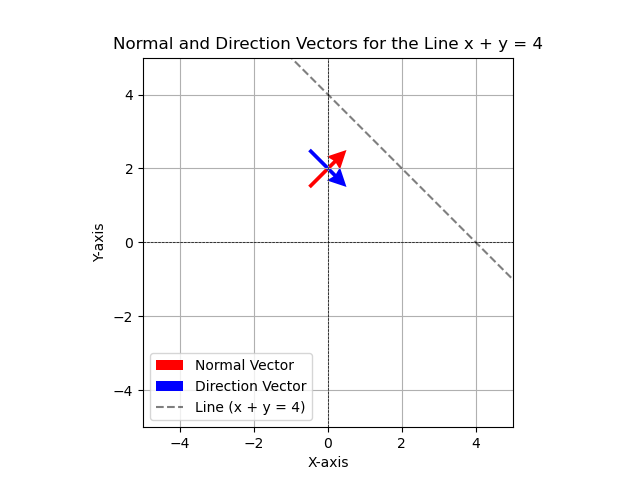
\includegraphics[width=0.5\linewidth]{Figures/Figure_1.png}
    \caption{Caption}
    \label{fig:enter-label}
\end{figure}

\end{document}

